\section[Probability Weighting]{What are weighting for? A mechanistic explanation of probability weighting}
\subsection{Main Result}

\begin{frame}{Main results}
\begin{center}
	\includegraphics[width=.9\textwidth]{../../img/papers/PW-Gaussian_vs_KT}
\end{center}
\begin{enumerate}
	\item	generic inverse-S shape can be explained by difference in uncertainty
	\item process of estimation of this uncertainty generates inverse-S shape
% 	\item	relative estimation error in $p(x)$ is greater for rarer events 	
\end{enumerate}
\label{MainResults}
\hyperlink{weight_vs_estimate}{\beamergotobutton{PW K\&T 1979}}
\end{frame}

\subsection{Probability Weighting}

\begin{frame}{Probability Weighting (PW)}

\begin{columns}[T]
\column{0.5\textwidth}
% \begin{center}
	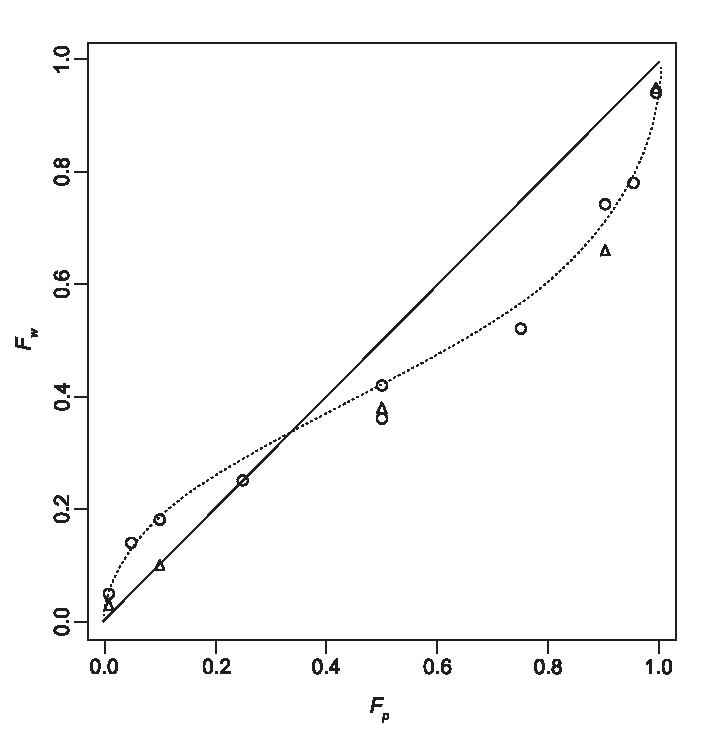
\includegraphics[width=.9\textwidth]{img/TK1992.pdf}
% \end{center}

\parencite[p. 310, Fig. 1,relabelled axes]{TverskyKahneman1992}

\column{0.5\textwidth}
\begin{itemize}
  \item overestimation of rare events $\rightarrow$ underestimation of common events
  \item stable empirical pattern: inverse-S shape
\end{itemize}

\red{Received wisdom:}
\bi
	\item	\red{PW = maladaptive irrational cognitive bias}
\ei

\begin{block}{In search of a mechanism}
	\begin{itemize}
	  \item[$\hookrightarrow$] How does this pattern emerge?
  	\item[$\hookrightarrow$] Can we derive the functional form (rather than merely fitting some function)?
	\end{itemize}
\end{block}

\end{columns}
\end{frame}

\begin{frame}{Set up : A Thought Experiment}
\begin{columns}[T]
\column{0.5\textwidth}
	\centering
	\textbf{Disinterested Observer (DO)} \\
	\vspace{0.5em}
% 	\includegraphics[width=.9\textwidth]{../../img/people/TverskyKahneman} \\
	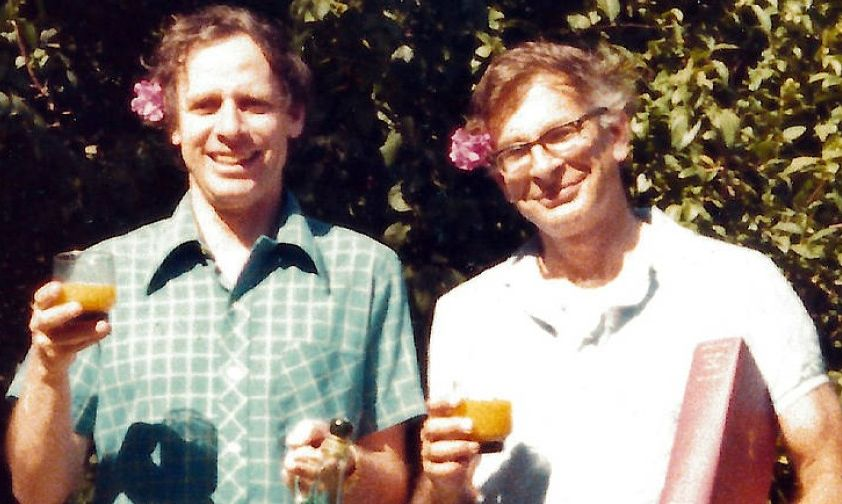
\includegraphics[height=3cm]{../../img/people/TverskyKahnemanFunny} \\
	\vspace{0.5em}
\column{0.5\textwidth}
	\centering
	\textbf{Decision Maker (DM)} \\
	\vspace{0.5em}
	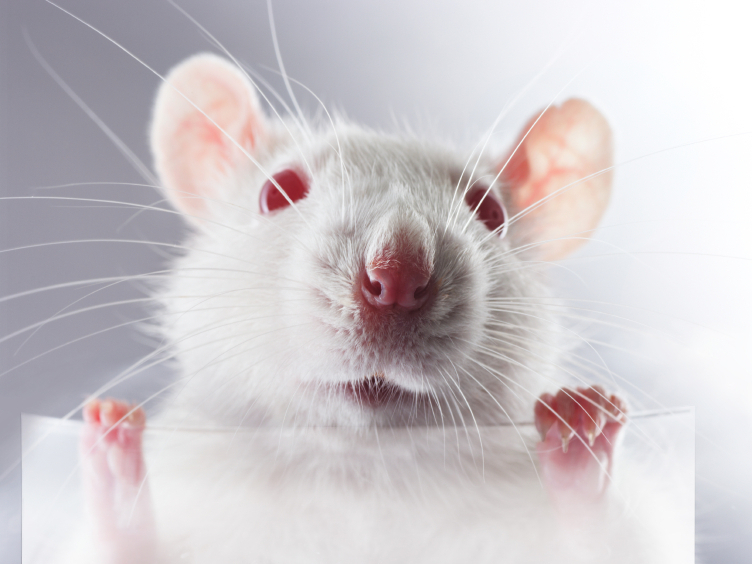
\includegraphics[height=3cm]{../../img/LabRat} \\
	\vspace{0.5em}
\end{columns}

\begin{columns}[T]
\column{0.05\textwidth}
\column{0.35\textwidth}
	\vspace{0.5em}
% 	\centering
	DO has a \red{model} of the random variable $X$, \eg payout of a gamble \\
	\red{probabilities $p(x)$} \\
  \red{CDF $F_p(x)$}\\
\column{0.2\textwidth}
\centering
	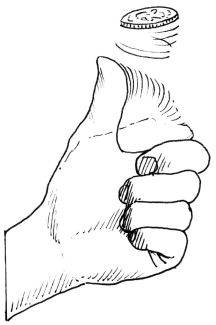
\includegraphics[height=3cm]{../../img/cartoons/coinflip}
\column{0.4\textwidth}
	\vspace{0.5em}
% 	\centering
  DM has a \blue{different model} of the same random variable $X$ with greater uncertainty\\
   \blue{decision weights $w(x)$} \\
   \blue{CDF $F_w(x)$}
\end{columns}
\end{frame}

\subsection{Location and Scale of PDFs}
% \hyperlink{t-distribution}{\beamergotobutton{HTD}}
% Transmission of different uncertainties from PDFs into CDFs}

\begin{frame}{Types of Different Uncertainties}
\centering
	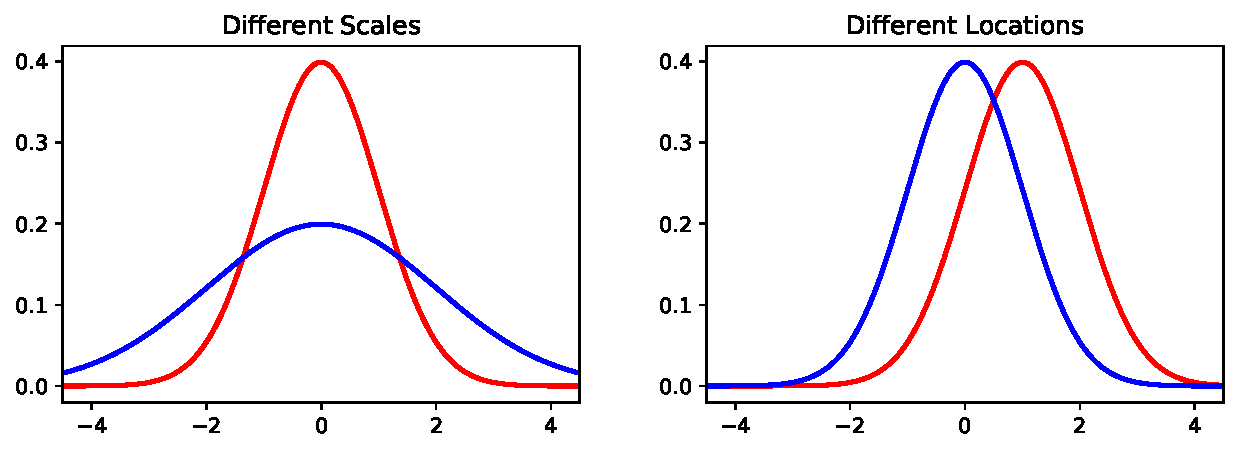
\includegraphics[width=0.8\textwidth]{img/2GaussianPDFs2Scales2Locations.pdf}
	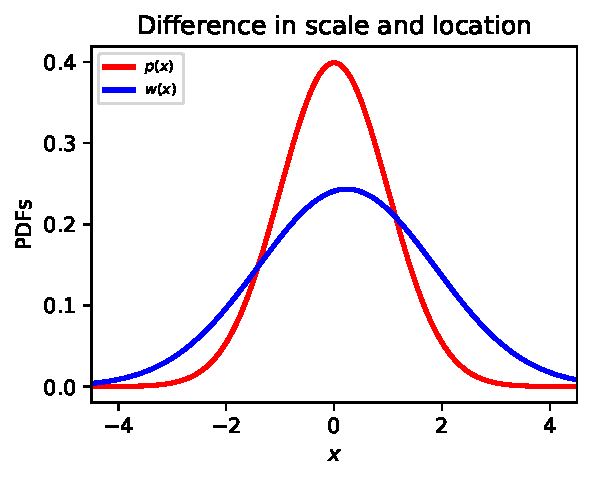
\includegraphics[width=0.4\textwidth]{img/mapping_pdfs_diff_scale_loc.pdf}
\end{frame}

\begin{frame}{Transmission of Different Uncertainty from PDF in CDF
 \hyperlink{diffShapes}{\beamergotobutton{Algo}} }
\centering
	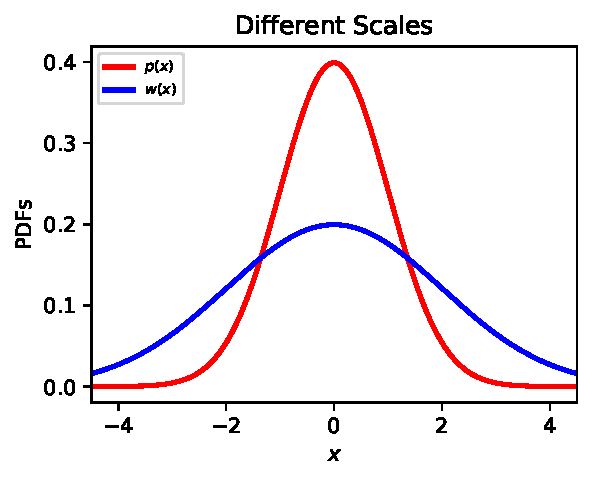
\includegraphics[width=0.4\textwidth]{img/2GaussianPDFs2Scales.pdf}
	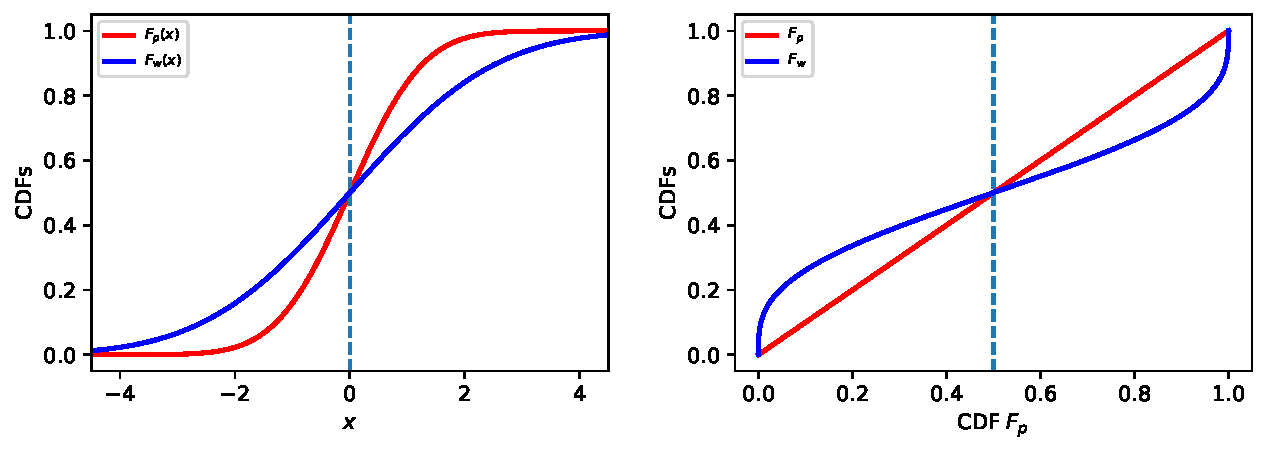
\includegraphics[width=0.8\textwidth]{img/mapping_cdfs_noarrows.pdf}
\end{frame}

\begin{frame}{Combining Difference in Location and Scale leads to Inverse S}
\centering
	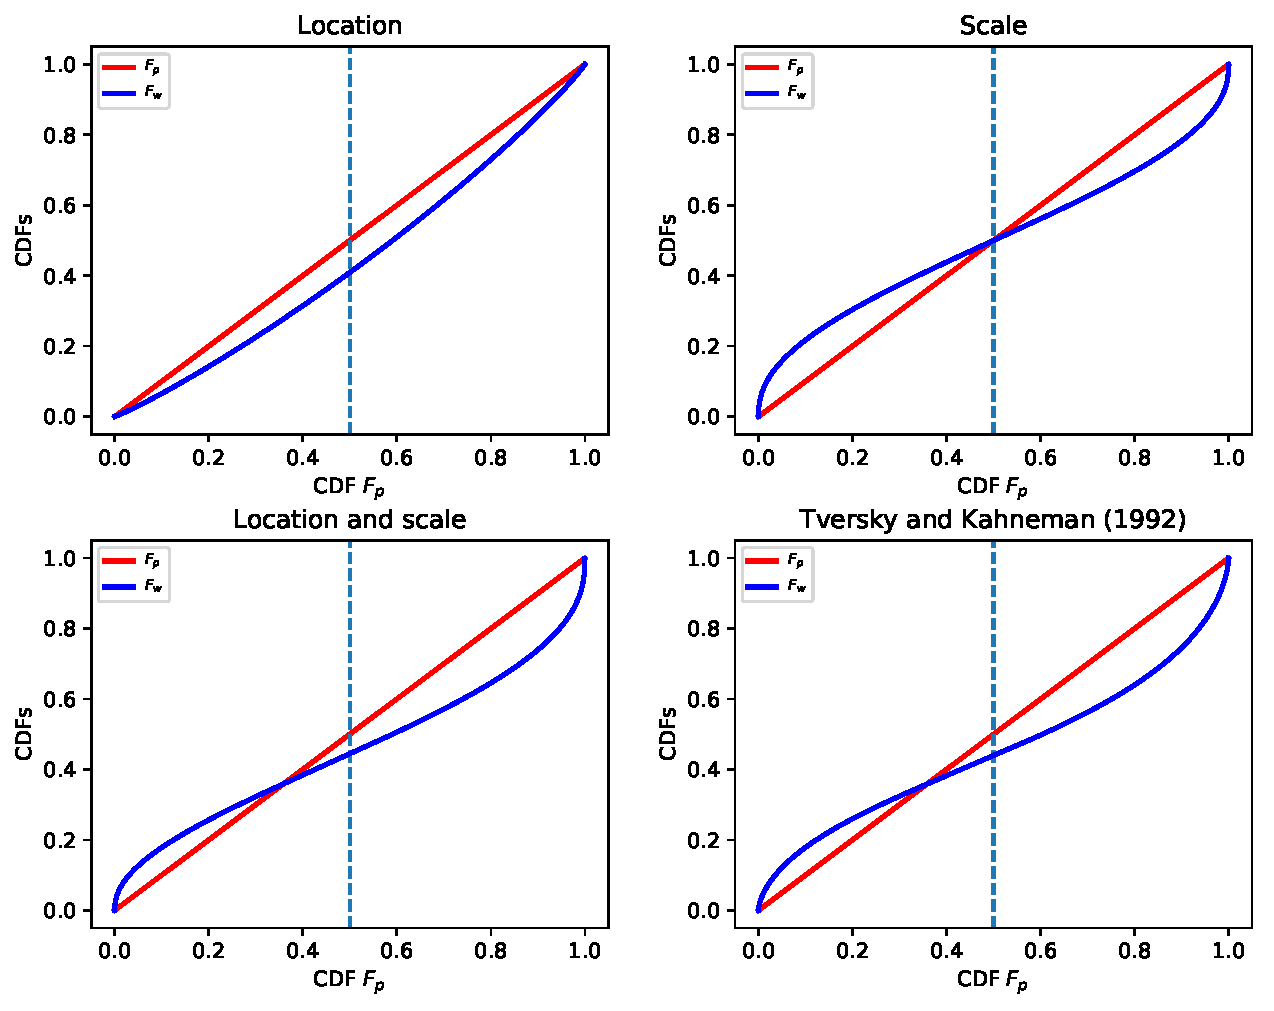
\includegraphics[width=0.78\textwidth]{img/Gauss_scale_location_both_KT.pdf}
	\label{LocationScale}
\end{frame}

\begin{frame}{Interim conclusion}
\bi
	\item greater scale reproduces inverse-S shape
	\item differences in location and scale reproduce asymmetric inverse-S shape
	\item inverse-S shape arises for all unimodal distributions
	\item Probability Weighting is the effect of a difference in uncertainty
	\item[]
	\item[] \textit{Job done. Thank you for your attention ;)}
	\hfill
	\hyperlink{FunctionalForms}{\beamergotobutton{Functional Forms}}
	\label{InterimConclusion}
\ei
	\vspace{2em}
	\centering
	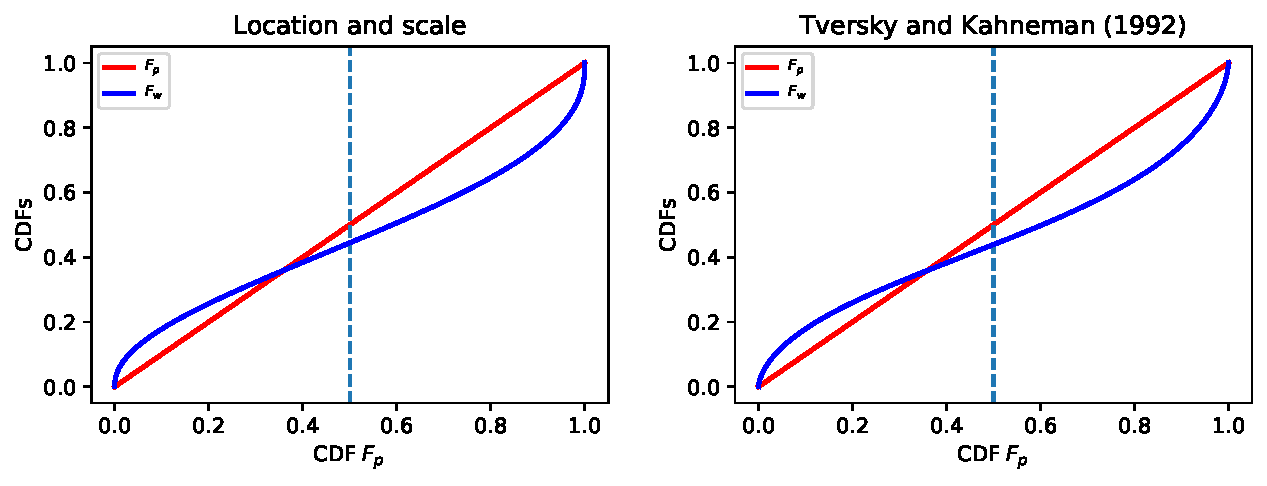
\includegraphics[width=0.8\textwidth]{img/Our_result_and_KT.pdf}
\end{frame}

\subsection{Ergodicity Question}

\begin{frame}{Asking the Ergodicity Question}
\begin{columns}[T]
\column{.35\textwidth}
	\bc \textbf{DO's concern} \ec
	What happens on average to the \red{ensemble} of subjects?
\column{.02\textwidth}
\centering \vspace{3em} \\ \red{\large $\neq$}
\column{.49\textwidth}
	\bc \textbf{DM's concern} \ec
	What happens to me \blue{on average over finite time}?
	\bi
	  \item DM's adaptive/ecological rationality $\equiv$ survival, \ie evolutionary incentive to err on the side of caution
	  \item[$\rightarrow$] add more uncertainty to his model
	\ei
\end{columns}
\end{frame}


\begin{frame}{Extra Uncertainty is Part of DM's Inference Problem}
% DM's extra uncertainty in the random variable $X$:
\begin{itemize}
	\item ``probability'' is polysemous \quelle{\parencite{Gigerenzer1991,Gigerenzer2018,HertwigGigerenzer1999}}
  \item probabilities are not observable, but
  \item DM experiences a trajectory of events and 
  \item counts of (rare) events are observable
  \item[$\hookrightarrow$] \textbf{DM's inference problem:} estimate probability $p(x)$ from counts
\end{itemize}

\vspace{1em}
Furthermore \ldots
\begin{itemize}
  \item DM has no control over the experiment,
	\item DM's incomplete comprehension of the experiment/decision problem,
	\item DM needs to trust the DO
	\item uncertain outcome is consequential only to the DM,
% 	\item DM's ignorance,
	\item \ldots
\end{itemize}
\end{frame}

\begin{frame}{Nature of Inference for Rare Events}
\begin{columns}[T]
\column{0.5\textwidth}
\textbf{Rare Event} \hfill \includegraphics[height=1.5cm]{../../img/Black-Swan-900} \hfill
\begin{itemize}
  \item asymptotic probability $p(x) = 0.001$
  \item time series of 100 observations
  \item $\sim 99.5\%$ of such time series will contain 0 or 1 events
  \item Na\"ive estimation: $\phat(x) = 0$ or $\phat(x)=0.01$, \ie either impossible or ten times more frequently than actual frequency
\end{itemize}
\column{0.5\textwidth}
\textbf{Common Event} \hfill 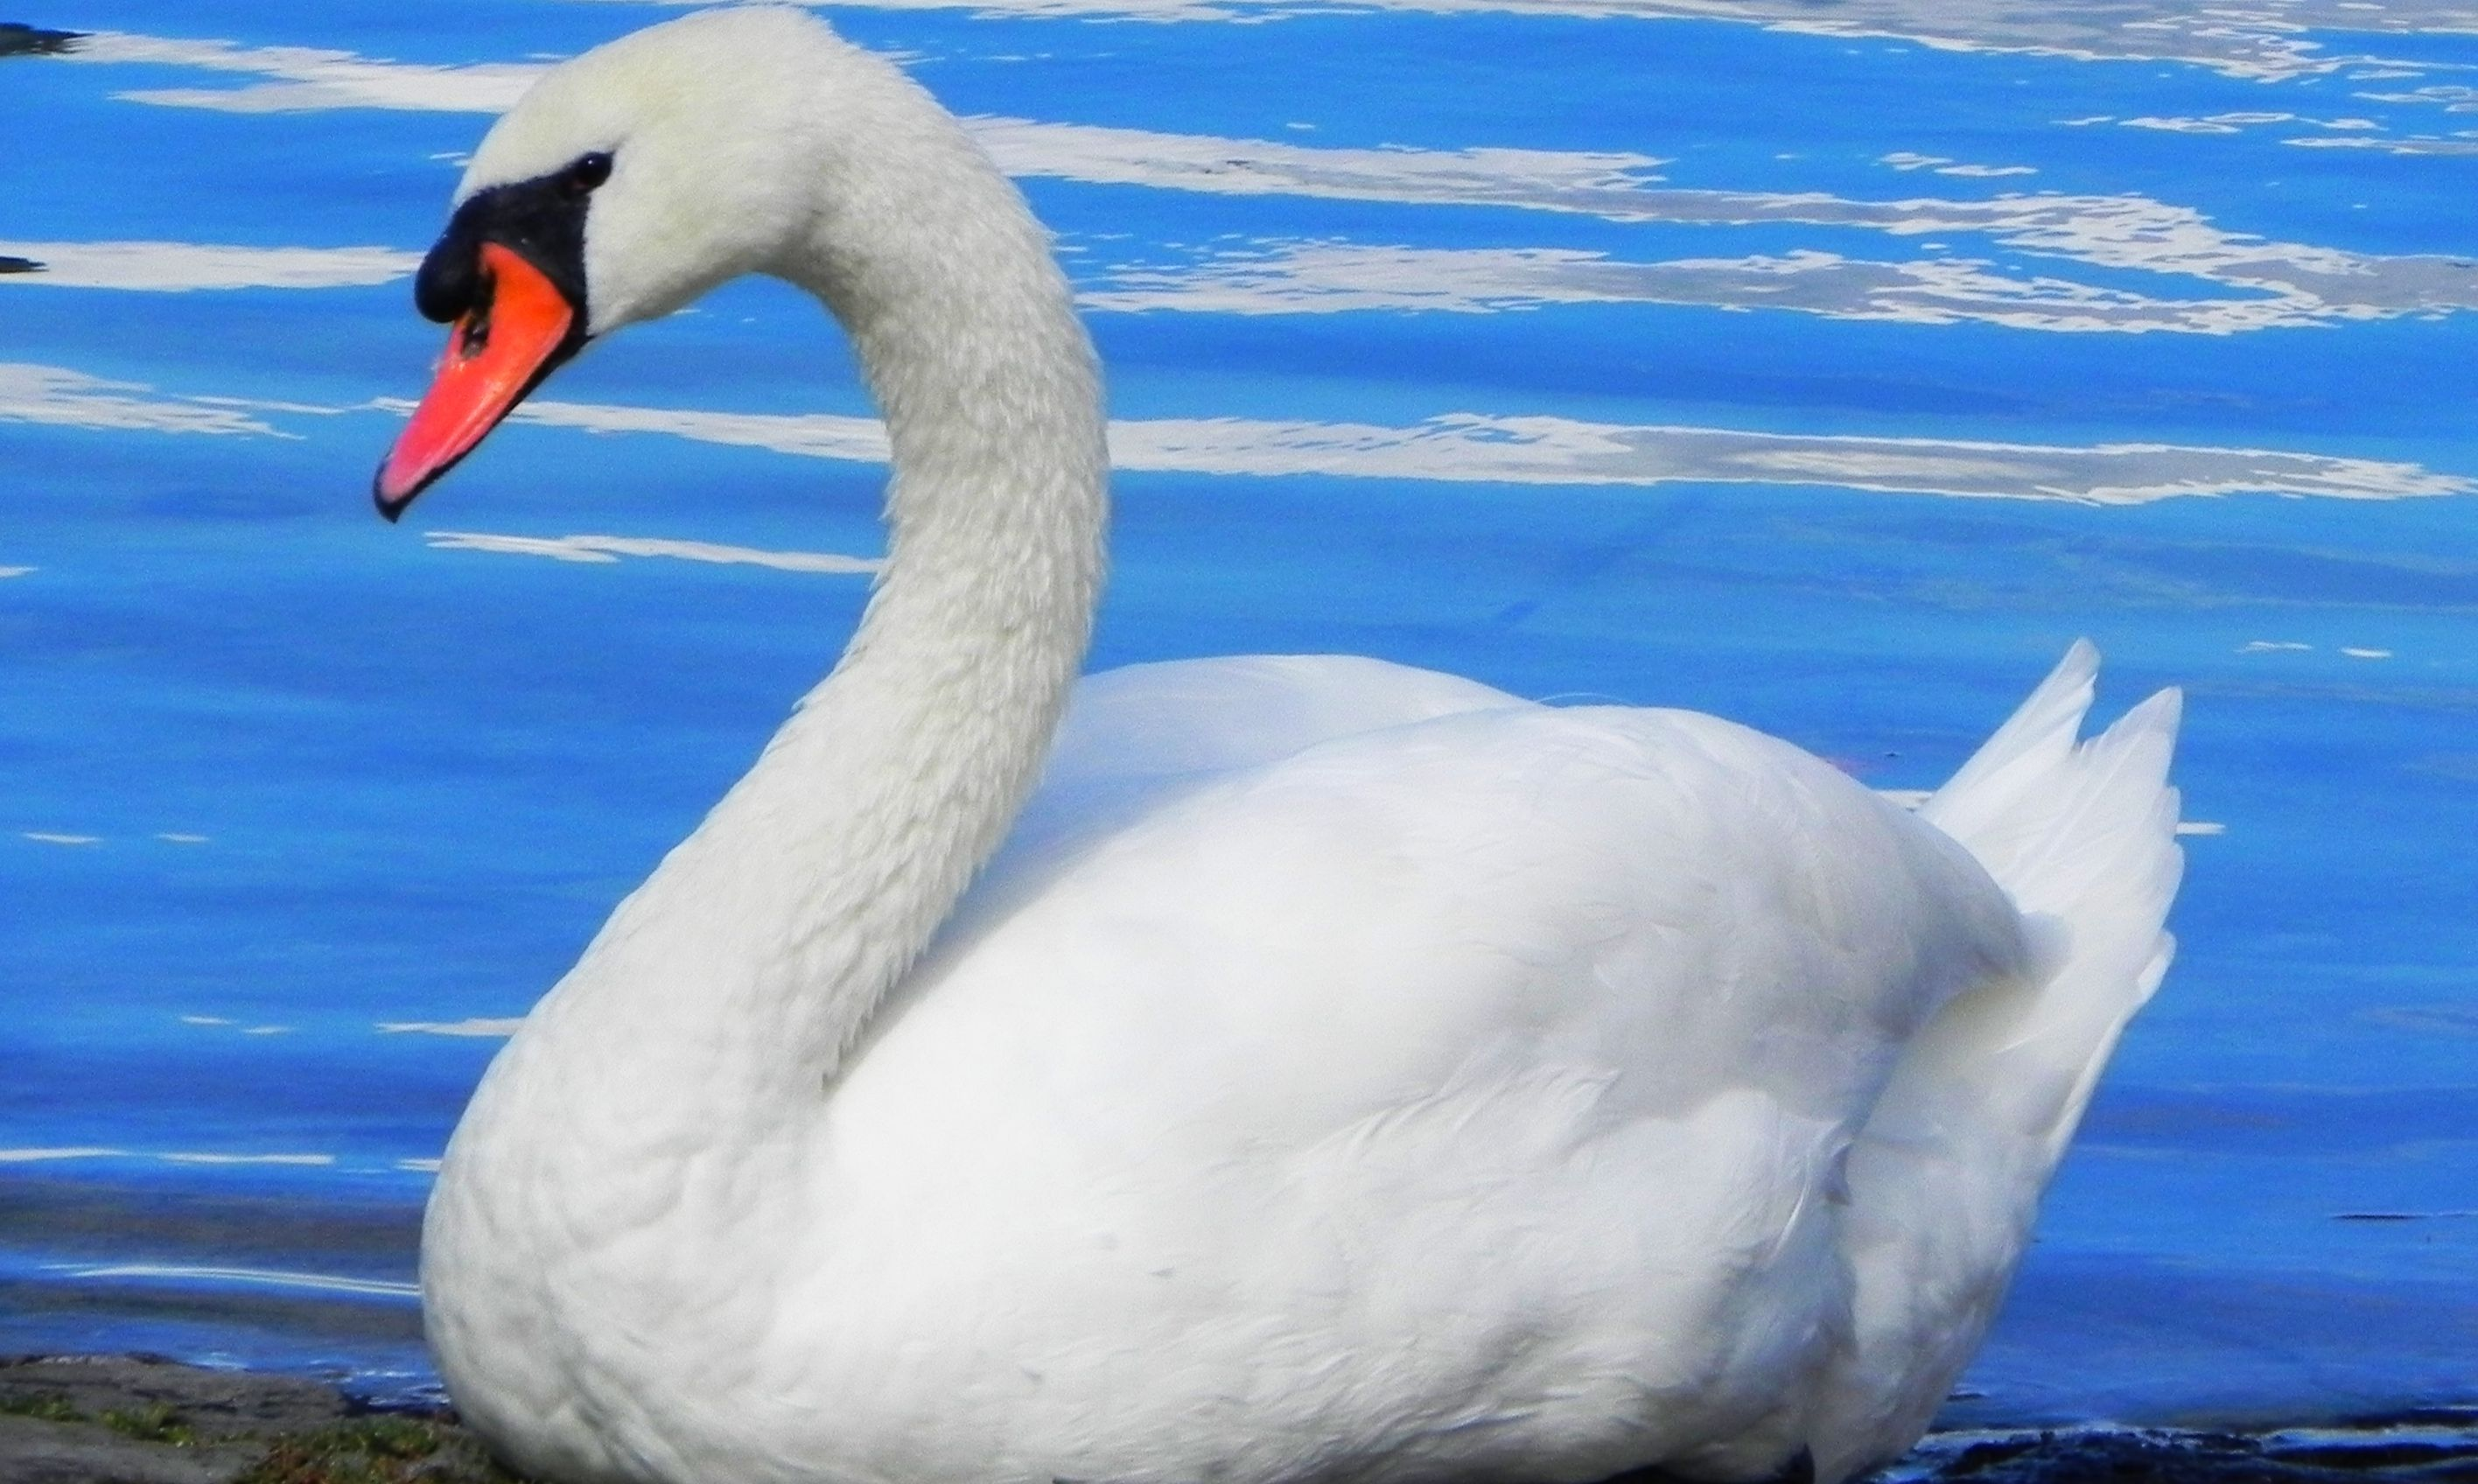
\includegraphics[height=1.5cm]{../../img/WhiteSwan}  \hfill
\begin{itemize}
  \item asymptotic probability $p=0.5$
  \item time series of 100 observations
  \item $\sim 99.5\%$ of time series would contain between 35 and 65 events,
  \item leading to a much smaller relative error in probability estimates
\end{itemize}
\end{columns}
\vspace{2em}
% \centering
$\hookrightarrow$ the smaller $p(x)$ the smaller the count of it in a finite time series \\
$\hookrightarrow$ the bigger the relative estimation error
\end{frame}

\begin{frame}{Relative Estimation Error is Larger for Rarer Events}

relative estimation errors scales like $\nicefrac{1}{\sqrt{\text{count}}}$

\begin{center}
\begin{table}[!htb]
  \begin{tabular}{@{}ccccc@{}}
\toprule[2pt]
\makecell{Asymptotic\\probability} & \makecell{Most likely\\count} & \makecell{Standard error\\in count} & \makecell{Standard error\\in probability} & \makecell{Relative error\\in probability}\\
\midrule[2pt]
% .5 &	5000 & 71	& 0.01 & 0.71\%\\
0.1 & 1000 & 32 & 0.003 & 3\%\\
0.01 & 100 & 10 & 0.001 & 10\%\\
0.001 & 10 & 3 & 0.0003& 30\%\\
0.0001 & 1 & 1 & 0.0001 &100\%\\
\bottomrule[2pt]
\end{tabular}
\caption{This table assumes $T = 10000$ observed time intervals. To be read as follows (first line): for an event of asymptotic probability 0.1, the most likely count in 10000 trials is 1000. Assuming Poisson statistics, this comes with an estimation error of $\sqrt{1000} = 32$ in the count and $32/10000 = 0.003$ in the probability, which is $0.003/0.1=3\%$ of the asymptotic probability.}
\label{errors}
\end{table}
\end{center}
\end{frame}


\subsection{Estimation}

% \begin{frame}{Simulation of the Estimation}
% \begin{center}
% 	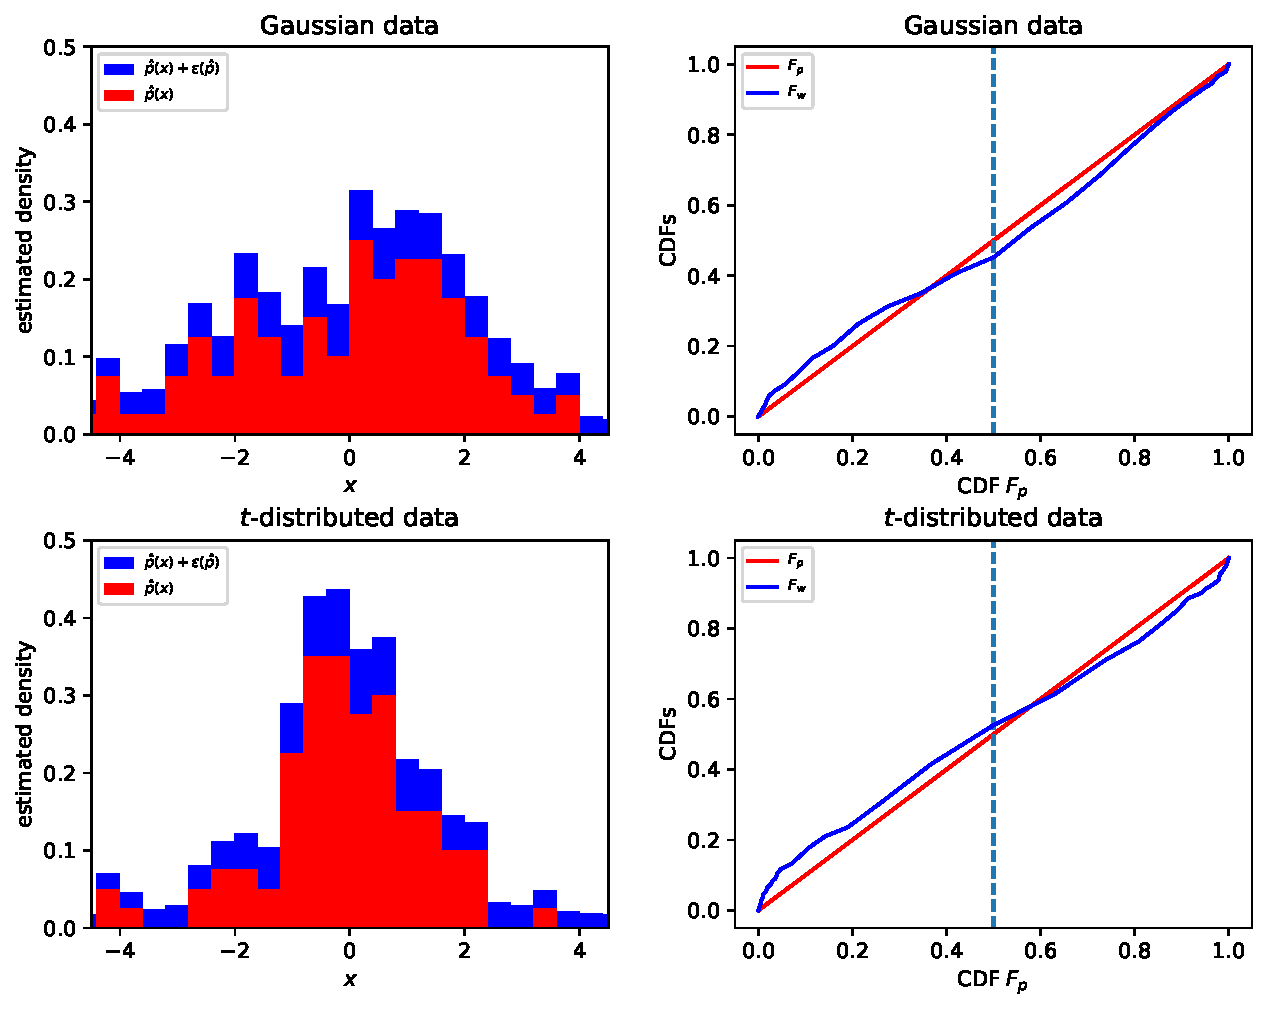
\includegraphics[width=.65\textwidth]{img/dm_count_sim} \\
% 	$T = 100$, estimates of \red{$\phat(x)$} in red, estimates with one standard error \blue{$\phat(x) + \err{\phat(x)}$} in blue 
% \end{center}
% 
% \end{frame}
% 
% \begin{frame}
% 	Using the fact that $n(x)$ is a random variable itself, $n(x) \sim Poisson$, its fluctuations scale like $\sqrt{n(x)}$ \\
% 
% 	Using the count $n(x)$ to infer the asymptotic PDF as
% 	\begin{align}	  
% 		p(x)	&\approx \frac{n(x)}{T\delta x} \pm \frac{\sqrt{n(x)}}{T \delta x} \\
% 					&\approx \phat(x) \pm \err{\phat(x)}
% 	\elabel{prob_est}
% 	\end{align}
% 	with the standard error (expressed in terms of the estimate itself)
% 	$$\err{\phat(x)} \equiv \frac{\sqrt{n(x)}}{T \delta x} = \sqrt{\frac{\phat(x)}{T \delta x}}$$
% 	\bi
% 		\item standard error $\err{\phat(x)}$ shrinks as the probability decreases
% 		\item relative error in the estimate is $1/\sqrt{\phat(x)T\delta x}$ grows as the event becomes rarer
% 		\item consistent with our claim, that low probabilities come with larger relative errors
% 		\item[$\hookrightarrow$] Errors in probability estimates behave differently for low probabilities than for high probabilities: absolute errors are smaller for lower probabilities, but relative errors are larger
% 	\ei
% \end{frame}

% \begin{frame}{Ergodicity Economics Research Programme}%{Everything happens over time}
% ?
% \end{frame}

% \begin{frame}{}
% 
% \end{frame}
% 
% \begin{frame}{}
% 
% \end{frame}
% 
% \begin{frame}{}
% 
% \end{frame}
% 
% 
% \begin{frame}{}
% 
% \end{frame}

\subsection{Conclusion}

\begin{frame}{Conclusion}
\lmlblue{Ergodicity Economics explains probability weighting}
\begin{itemize}
  \item we find an inverse-S shape as a neutral indicator of a difference in opinion
%   \item relative probability estimation errors are greater for rarer events
	\item we find that quite generally the relative uncertainties are larger for rare events than for common events, which generates the inverse-S shape
  
  \item[$\hookrightarrow$] Probability weighting is rational cautious behaviour under uncertainty
  \item[]
  \item See full paper at \url{bit.ly/lml-pw-r1}
  \item links to play with the code are inside
%   \\ \fullcite{PetersETAL2020R1}
% 	\item See blog post for the basic reasoning \fullcite{Peters2020}
% 	\item See blog post for the basic reasoning \fullcite{Buchanan2020}
\end{itemize}

\end{frame}
